\documentclass[11pt,a4paper]{article}
\usepackage[margin=2.1cm]{geometry}
\usepackage{fontspec}
\usepackage{amsmath}
\usepackage{unicode-math}
\setmainfont{texgyretermes}[Extension=.otf, UprightFont=*-regular, BoldFont=*-bold, ItalicFont=*-italic, BoldItalicFont=*-bolditalic]
\setmathfont{texgyretermes-math.otf}
\usepackage{graphicx}
\usepackage{booktabs}
\usepackage{tabularx}
\usepackage{multicol}
\usepackage[font=small,labelfont=bf,skip=4pt]{caption}
\usepackage{xcolor}
\usepackage{tikz}
\usetikzlibrary{arrows.meta,positioning,calc}
\usepackage{enumitem}
\usepackage{placeins}
\usepackage{float}
\emergencystretch=1.5em
\usepackage{microtype}
\usepackage[colorlinks=true,linkcolor=blue!50!black,citecolor=blue!50!black,urlcolor=blue!60!black]{hyperref}
\hypersetup{pdftitle={Predicting Sparse HRTF Reconstruction Error from Sampling Geometry: Coverage, Conditioning and Transfer from HUTUBS to SADIE II},pdfauthor={Fanxing Ning}}

\graphicspath{{../figures/pdf/}}
\setlist{nosep,leftmargin=1.3em}
\setlength{\parskip}{0pt}
\usepackage{titlesec}
\titlespacing*{\section}{0pt}{2.2ex plus .6ex minus .2ex}{1.0ex plus .2ex}
\titlespacing*{\subsection}{0pt}{1.6ex plus .5ex minus .2ex}{0.7ex plus .2ex}
\setlength{\textfloatsep}{10pt plus 2pt minus 2pt}
\setlength{\floatsep}{8pt plus 2pt minus 2pt}
\renewcommand{\topfraction}{0.92}
\renewcommand{\bottomfraction}{0.6}
\renewcommand{\textfraction}{0.08}
\renewcommand{\floatpagefraction}{0.85}
\setcounter{topnumber}{3}
\setcounter{bottomnumber}{2}
\setcounter{totalnumber}{4}
\newcommand{\us}{\,\textmu s}
\newcommand{\dmin}{d_{\min}}
\newcommand{\rmax}{r_{\max}}
\newcommand{\repo}{https://github.com/ningfanxing-sys/elec5305-project-540084782}
\newcommand{\site}{https://ningfanxing-sys.github.io/elec5305-project-540084782}

\begin{document}

\begin{center}
{\Large\bfseries Predicting Sparse HRTF Reconstruction Error from Sampling Geometry:\\[1pt]
Coverage, Conditioning and Transfer from HUTUBS to SADIE~II\par}
\vspace{5pt}
{\large Fanxing Ning (SID 540084782)}\\[1pt]
ELEC5305 Speech and Audio Processing, The University of Sydney, November 2026\\[3pt]
\small GitHub repository: \href{\repo}{\nolinkurl{https://github.com/ningfanxing-sys/elec5305-project-540084782}}\\
\href{\site/}{Project site}\enspace$\cdot$\enspace \href{\site/video/}{Video presentation}\enspace$\cdot$\enspace \href{\site/demo/}{Binaural listening examples}
\end{center}

\begin{abstract}
\noindent Dense individual head-related transfer functions (HRTFs) are usually reconstructed from sparse measurements. This project asks how well the coverage and spherical-harmonic (SH) conditioning of a sparse layout predict the reconstruction error, and whether these relationships transfer from HUTUBS to SADIE~II. Dense HRTF sets were reconstructed from shared layouts of 25, 50 and 100 measured directions by nearest-neighbour (NN), SH, time-aligned SH and ridge-regularised time-aligned SH interpolation, with SUpDEq magnitude correction (MCA) as a published reference; orders and ridge parameters were frozen on half of HUTUBS. Adding the distance to the nearest measured direction to the number of directions raises the explained per-target error variance on HUTUBS from at most 7\% to 24--47\%, and for NN and SH the databases agree within 0.5~dB in every $5^\circ$ distance bin from $5^\circ$ to $30^\circ$. The covering radius ranks the 95th-percentile error (Spearman $\rho=0.95$--$0.96$ for NN). Above a condition number of about 10, unregularised SH errors grow by 4--7~dB per decade; ridge regularisation with $\lambda=0.01$--$0.1$ cuts the excess error of time-aligned SH at the highest order from 8.7 to 0.6~dB on the selection half and lowers the held-out error by 0.6--0.7~dB at the frozen order. On SADIE~II all four slopes keep their sign, three changing by 11--19\% and the time-aligned $\kappa$ slope by 72\%, so the form of each relationship transfers while its slope must be refitted. Time alignment brings the interaural time difference error on HUTUBS to 14\us{} (NN: 79\us) but helps much less on SADIE~II, whose onset estimates are about four times rougher; MCA helps in both databases, most on the contralateral side.
\end{abstract}

\begingroup\small
\setlength{\columnsep}{22pt}
\begin{multicols}{2}
\setcounter{tocdepth}{1}
\tableofcontents
\end{multicols}
\endgroup

%=====================================================================
\section{Introduction}

A head-related transfer function (HRTF) describes how the head, torso and outer ears filter sound before it reaches each ear drum. Binaural rendering needs dense, individual HRTFs, but measuring hundreds of directions takes specialist equipment and a long session~\cite{li2020}. Sparse measurements are therefore expanded into dense sets, usually by spherical-harmonic (SH) interpolation~\cite{evans1998,duraiswami2004,romigh2015}.

Sparse-reconstruction studies compare methods mainly by errors averaged over directions or regions~\cite{benhur2019,arend2021,arend2023,thuillier2024}. Such results do not show how the location of large errors depends on the measured layout, and the number of measured directions describes neither the coverage nor the stability of the SH fit. Bau et al.\ linked the best SH order mainly to the grid~\cite{bau2022}, leaving open which layout property predicts the error at each direction. Transfer to another database also needs testing, because measurement chains make databases differ systematically~\cite{andreopoulou2015,wen2023}.

This project relates the errors to three descriptors known before measurement: the distance $\dmin$ to the nearest measured direction, the covering radius $\rmax$ and the SH condition number $\kappa$ (Figure~\ref{fig:maps}). Shared nominal layouts were realised on HUTUBS~\cite{brinkmann2019} and SADIE~II~\cite{armstrong2018}. Time-aligned SH was reproduced, checked against SUpDEq~\cite{supdeq} and modified with ridge regularisation, whose benefit $\kappa$ predicts. Orders and ridge parameters were frozen on HUTUBS before the SADIE~II transfer test.

\begin{center}
\colorbox{black!5}{\parbox{0.95\linewidth}{\vspace{3pt}
\emph{Research question.} To what extent do the coverage and SH conditioning of a sparse measurement layout predict the error of sparse-to-dense HRTF reconstruction, and which of these relationships transfer from HUTUBS to SADIE~II?\\[2pt]
\emph{Secondary question.} How do time alignment and magnitude correction change the relationship between sampling geometry and error?\vspace{3pt}}}
\end{center}

\begin{figure}[t]
\centering
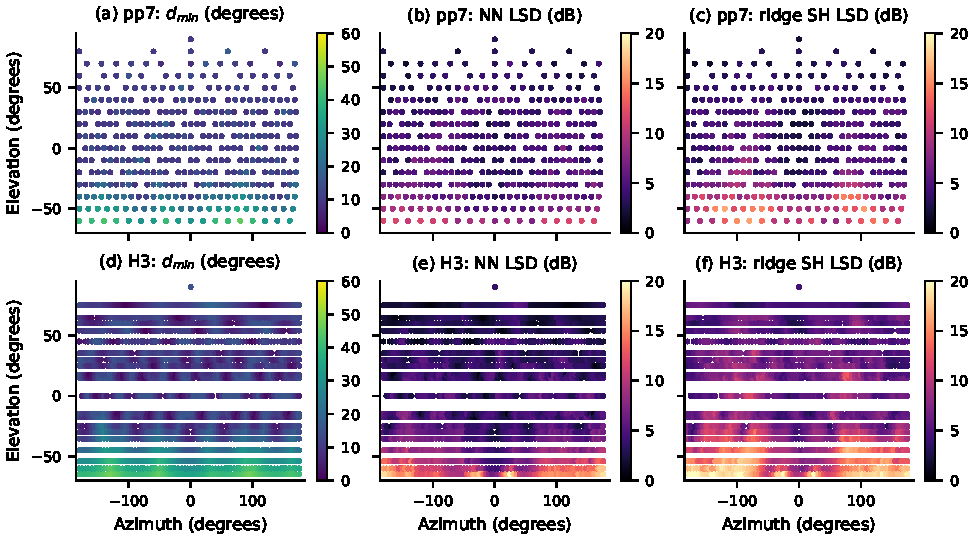
\includegraphics[width=\linewidth]{error_maps}
\caption{\textbf{Reconstruction error follows the distance to the nearest measured direction, in the same place in both databases.} Gap layout with $M=50$ (no measured directions below $-30^\circ$) on HUTUBS pp7 (a--c) and SADIE~II H3 (d--f): distance $\dmin$ to the nearest measured direction (a, d), NN error (b, e) and SH-aligned-ridge error (c, f) as log-spectral distortion (LSD, 200~Hz--16~kHz). Crosses mark the measured (context) directions.}
\label{fig:maps}
\end{figure}

The project makes four contributions:
\begin{itemize}
\item shared 25-, 50- and 100-direction layouts realised on three measured grids (Section~\ref{sec:methods});
\item evidence that coverage predicts where errors are large, explaining several times more variance than the number of directions (Section~\ref{sec:coverage});
\item evidence that $\kappa$ predicts when SH fitting amplifies errors and when ridge regularisation pays off (Section~\ref{sec:kappa});
\item a frozen transfer test, with listening examples, that separates the geometric relationships from the database-dependent alignment step (Sections~\ref{sec:transfer}--\ref{sec:listening}).
\end{itemize}

%=====================================================================
\section{Literature Review}
\label{sec:lit}

\subsection{HRTF cues, measurement and databases}

HRTFs carry interaural time differences (ITDs), interaural level differences (ILDs) and monaural spectral cues, mainly from the pinna. The low-frequency ITD dominates horizontal localisation~\cite{wightman1992}, while neither the interaural spectral difference nor one ear's spectrum alone sufficed for accurate elevation judgements~\cite{jin2004}; spectral and interaural errors are therefore reported separately.

CIPIC~\cite{algazi2001}, SYMARE~\cite{jin2014}, HUTUBS~\cite{brinkmann2019}, SADIE~II~\cite{armstrong2018} and SONICOM~\cite{engel2023} use SOFA~\cite{majdak2022}, but differ in grid, distance, equalisation and processing. Round-robin measurements of the same mannequin differed between laboratories~\cite{andreopoulou2015}, and Wen et al.\ classified HRTFs by database, attributing this to measurement setups~\cite{wen2023}. Relationships therefore need cross-database tests.

\subsection{Spherical-harmonic interpolation of sparse sets}

SH interpolation fits a finite expansion to the measured directions and evaluates it anywhere on the sphere~\cite{evans1998,duraiswami2004,romigh2015}. Because the spatial complexity of the HRTF grows with frequency~\cite{zhang2010}, a sparse budget forces truncation: order $N$ holds up to the spatial aliasing frequency $f_A=Nc/(2\pi r)$ for head radius $r$~\cite{rafaely2019,arend2023}, about 1.2, 2.5 and 3.7~kHz for $N=2$, 4 and 6 with $r=8.75$~cm, and truncation smooths pinna detail and lowers high-frequency energy~\cite{benhur2017}. An order too high for the grid instead makes the fit ill-conditioned and amplifies noise and unmodelled detail~\cite{rafaely2019}. Spherical Marcinkiewicz--Zygmund inequalities link coverage and conditioning: weighted least squares stays stable while the largest gap of the sampling set (its mesh norm) is small compared with the angular resolution of order $N$~\cite{mhaskar2001}.

Zotkin et al.\ applied Tikhonov (ridge) regularisation to SH fits on incomplete grids~\cite{zotkin2009}. Bau et al.\ found that the optimal order depends mainly on the grid and the regularisation, hardly on the HRTF set, and selected it by interpolating a reference HRTF set on the same grid~\cite{bau2022}. This motivates testing whether grid descriptors predict the error at each direction across measurement chains.

\subsection{Time alignment, equalisation and magnitude correction}

Removing the direction-dependent time of arrival (TOA) before the fit lowers the effective SH order~\cite{evans1998,arend2021}. Arend et al.\ found similar results for four such pre-processing methods except at low orders and for contralateral directions, with an order of about 7 transparent for a frontal speech source~\cite{arend2021}. Onset-based alignment relies on numerically estimated delays; Ben-Hur et al.\ proposed a parametric ear alignment that is more robust to measurement noise~\cite{benhur2019}, and Pörschmann et al.\ equalised each HRTF by a rigid-sphere transfer function before the fit (SUpDEq)~\cite{porschmann2019}. A later magnitude correction (MCA) reduced simulated high-frequency errors by up to 1.5~dB over all directions and 4~dB contralaterally and improved ILDs~\cite{arend2023}. For onset-based alignment the estimator matters: ITD estimates differ substantially between methods~\cite{katz2014}.

The spherical neural-process meta-learner of Thuillier, Jin and Välimäki reduced the relative interpolation error by up to 3~dB and the number of points needed by up to nearly half, and its calibrated uncertainty could guide further measurements~\cite{thuillier2024}. Neural fields have represented HRTFs with different sampling schemes in one model~\cite{zhang2023}. These models need training data and a learned prior, whereas the descriptors studied here locate unreliable regions from the layout alone.

\subsection{Approaches and available code}

Table~\ref{tab:approaches} compares the approaches. SUpDEq~\cite{supdeq}, the reference implementation of~\cite{arend2023}, provides interpolators, alignment, Tikhonov regularisation and MCA, and was run unchanged. NN and three SH variants were implemented in Python to expose the matrix, singular values, weights and per-target errors of every fit, and cross-checked against SUpDEq (Section~\ref{sec:mca}); their dependence on geometry can be examined without training.

\begin{table}[t]
\centering
\caption{Approaches to sparse HRTF reconstruction and their role in this project.}
\label{tab:approaches}
\footnotesize
\setlength{\tabcolsep}{3.5pt}
\begin{tabularx}{\linewidth}{@{}>{\raggedright\arraybackslash}p{2.55cm}>{\raggedright\arraybackslash}X>{\raggedright\arraybackslash}X>{\raggedright\arraybackslash}p{2.25cm}>{\raggedright\arraybackslash}p{2.5cm}@{}}
\toprule
Approach & Strength & Limitation & Code & Role here \\
\midrule
Nearest neighbour (NN) & Keeps the measured spectrum; no fitting & Piecewise constant over direction & Trivial & Baseline \\
SH expansion~\cite{evans1998,romigh2015} & Continuous, compact, evaluable anywhere & Order limited by the budget; ill-conditioned on irregular grids & SUpDEq~\cite{supdeq}, spharpy~\cite{spharpy} & Own Python, with $\kappa$ and singular values \\
Ridge SH~\cite{zotkin2009,bau2022} & Stabilises ill-conditioned fits & Biases the coefficients; needs $\lambda$ & SUpDEq & Own Python; $N$, $\lambda$ chosen on HUTUBS \\
Onset time alignment~\cite{evans1998,arend2021} & Lowers the effective order; restores ITD & Relies on onset estimates & SUpDEq OBTA & Own Python and SUpDEq \\
Ear alignment, SUpDEq equalisation~\cite{benhur2019,porschmann2019} & Parametric; less sensitive to noise & Needs a head model & SUpDEq & Not used \\
Magnitude correction (MCA)~\cite{arend2023} & Corrects high-frequency and contralateral magnitude & Does not repair onset errors & SUpDEq & Published reference \\
Neural processes and fields~\cite{thuillier2024,zhang2023} & Learned prior; uncertainty & Training data; less interpretable & Authors' code & Not used \\
\bottomrule
\end{tabularx}
\end{table}

Five concepts used here were new to the author. Spherical-Voronoi quadrature approximates the integral under which SH functions are orthonormal. Singular-value decomposition explains amplification and ridge filtering~\cite{hansen1998}. Removing an onset removes linear phase, although onset and ITD remain different estimates~\cite{katz2014}. One-to-one grid matching is a Hungarian assignment problem~\cite{kuhn1955}, and $R^2$ on a second database measures out-of-sample prediction.

%=====================================================================
\section{Methods}
\label{sec:methods}

For each subject, layout and budget, every method reconstructs the remaining measured directions (targets) from a sparse set of measured directions (the context), and the errors are related to descriptors of the context alone (Figure~\ref{fig:overview}).

\subsection{Data and pre-processing}
\label{sec:data}

HUTUBS has 440 directions on 10$^\circ$ elevation rings at 1.47~m~\cite{brinkmann2019,hutubs}; excluding two dummy-head sets leaves 94 sets from 93 people. SADIE~II version 2-2 has 18 humans measured at 1.2~m on two grids (H3--H9 and H10--H20)~\cite{armstrong2018,sadie}. Both use 44.1~kHz, 256-tap head-related impulse responses (HRIRs), with coordinates, receiver order and delays from SOFA metadata~\cite{majdak2022}. HUTUBS is split into 49 selection and 45 held-out sets; Table~\ref{tab:data} gives subject IDs and retained direction counts.

Taking the first sample above 10\% of the peak as the onset gives the wrong ITD sign on SADIE~II, where a slow low-frequency rise crosses the threshold first in the weaker contralateral ear (Figure~\ref{fig:alignment}a), possibly from post-processing compensation~\cite{armstrong2018}. The rule used here applies a fourth-order 1~kHz high-pass filter, upsamples by 8 and uses a 20\% threshold; it gives no sign errors and the smallest median difference from the cross-correlation ITD on the horizontal planes of the three grids (33\us{} on average, against 46\us{} for 10\%). Of 467 SADIE~II subject--direction pairs whose onset ITD departs from a $\sin(\text{lateral angle})$ fit by more than 400\us, 460 lie below $-65^\circ$, so both databases were restricted to elevations of at least $-65^\circ$. Figure~\ref{fig:appendix} shows the three grids and this check over all directions.

\subsection{Sparse layouts and geometry descriptors}
\label{sec:layouts}

For each budget $M\in\{25,50,100\}$, \emph{uniform} is a Fibonacci lattice above $-65^\circ$~\cite{gonzalez2010}, \emph{random1} and \emph{random2} are uniformly random above $-65^\circ$, and \emph{gap} is a Fibonacci lattice above $-30^\circ$ that leaves the lower region unsampled, so coverage and conditioning vary at a fixed budget. Each layout was mapped one-to-one onto measured directions by solving the assignment problem that minimises the total great-circle distance~\cite{kuhn1955}. With $\angle(\cdot,\cdot)$ the great-circle angle, $\mathcal C$ the context and $\mathcal T$ the targets, the local and worst-case coverage are
\begin{equation}
\dmin(\Omega)=\min_{i\in\mathcal C}\angle(\Omega,\Omega_i),\qquad \rmax=\max_{\Omega\in\mathcal T}\dmin(\Omega).
\end{equation}
Conditioning (Section~\ref{sec:sh}) was evaluated at $N_{\mathrm{fit}}=\lfloor\sqrt{M/2}\rfloor-1$, about two directions per coefficient (orders 2, 4 and 6 for $M=25$, 50 and 100), and $N_{\max}=\lfloor\sqrt M\rfloor-1$, the highest order with no more coefficients than directions (orders 4, 6 and 9).

\subsection{Reconstruction methods}
\label{sec:sh}

For each ear and frequency $f$, the real SH expansion is
\begin{equation}
H(f,\Omega)\approx\sum_{n=0}^{N}\sum_{m=-n}^{n}a_{nm}(f)\,Y_{nm}(\Omega),
\end{equation}
with $(N+1)^2$ coefficients estimated by weighted ridge least squares,
\begin{equation}
\hat{\mathbf a}=\arg\min_{\mathbf a}\big\|\mathbf W^{1/2}(\mathbf Y\mathbf a-\mathbf h)\big\|_2^2+\lambda\|\mathbf a\|_2^2,
\label{eq:ridge}
\end{equation}
where $\mathbf Y$ is the $M\times(N+1)^2$ SH matrix, $\mathbf h$ the complex context HRTFs and $\mathbf W$ spherical-Voronoi areas normalised to $4\pi$. With the singular-value decomposition $\mathbf W^{1/2}\mathbf Y=\mathbf U\boldsymbol\Sigma\mathbf V^{\mathsf T}$, the solution is
\begin{equation}
\hat{\mathbf a}=\sum_{k}\frac{\sigma_k^2}{\sigma_k^2+\lambda}\,\frac{\mathbf u_k^{\mathsf T}\mathbf W^{1/2}\mathbf h}{\sigma_k}\,\mathbf v_k,\qquad \kappa=\frac{\sigma_{\max}}{\sigma_{\min}}.
\label{eq:filter}
\end{equation}
At $\lambda=0$, dividing by small $\sigma_k$ amplifies noise and the HRTF detail beyond order $N$; for a consistent system, the relative coefficient error is bounded by $\kappa$ times the relative data error~\cite{hansen1998}. Ridge suppresses components with $\sigma_k^2\ll\lambda$ and leaves those with $\sigma_k^2\gg\lambda$ almost unchanged. With an orthonormal basis and normalised weights the singular values are of order one, so $\lambda$ acts on the same scale for every layout.

Time alignment writes $H(f,\Omega)=\tilde H(f,\Omega)\,e^{-j2\pi f\tau(\Omega)}$, separating each ear's TOA $\tau$ from a residual $\tilde H$ that varies more smoothly with direction. The context onsets are removed before fitting $\tilde H$, and an order-3 SH fit interpolates $\tau$ to the targets before the delay is restored.

\emph{NN} returns the HRTF of the nearest context direction. \emph{SH} fits the complex HRTFs at $N_{\mathrm{fit}}$ with $\lambda=0$ (and up to $N_{\max}$ for the conditioning analysis), and \emph{SH-aligned} does the same after time alignment. The modification, \emph{SH-aligned-ridge}, adds the ridge penalty with $N$ and $\lambda$ selected on HUTUBS. SUpDEq~\cite{supdeq} (commit 877401f) ran in MATLAB with onset alignment at $N_{\mathrm{fit}}$, without (\emph{OBTA}) and with (\emph{MCA}) magnitude correction; MCA compares the interpolated equivalent-rectangular-bandwidth magnitudes of the context~\cite{slaney1998} with those of the aligned reconstruction and applies their ratio as a minimum-phase filter above the spatial aliasing frequency~\cite{arend2023}. SUpDEq ran on a ten-subject subset (Table~\ref{tab:data}) with the uniform and gap layouts at all budgets and was scored by the same Python code.

\subsection{Error measures}

The log-spectral distortion at one target direction and ear is
\begin{equation}
\mathrm{LSD}=\sqrt{\frac{1}{|\mathcal F|}\sum_{f\in\mathcal F}\Big(20\log_{10}\frac{|H(f)|}{|\hat H(f)|}\Big)^2},
\end{equation}
evaluated over 200~Hz--16~kHz and in the bands 0.2--1, 1--4, 4--8 and 8--16~kHz, and averaged over the ears unless stated otherwise. For the ear-side analysis, the lateral angle of the source towards the left ear is $\arcsin(\cos\theta\sin\phi)$ (azimuth $\phi$, elevation $\theta$) and its negative for the right ear, so $+90^\circ$ is ipsilateral and $-90^\circ$ contralateral. The ITD is the lag of the interaural cross-correlation, interpolated by a factor of 8 (2.8\us{} steps) and independent of the onset rule; the ILD is the broadband energy ratio of the ears. Every SH fit stores $\kappa$, the coefficient norm, the relative reconstruction energy and a finite-output flag.

\subsection{Protocol and analysis}
\label{sec:protocol}

For SH-aligned-ridge, every order up to $N_{\max}$ and every $\lambda\in\{0,10^{-5},\dots,10^{-1},1\}$ was scored on the 49 HUTUBS selection sets, and the pair with the lowest mean per-subject median LSD was frozen: orders 3/5/7 (uniform), 3/4/6 (random) and 4/6/8 (gap) for $M=25/50/100$, with $\lambda=0.1$ at $M=25$ and 50 and $\lambda=0.01$ at $M=100$. The transfer analysis compares the slopes of error against $\log_{10}\kappa$ and $\dmin$, with 95\% subject-bootstrap intervals, and the ranking of NN and SH-aligned-ridge in the 12 conditions, by the median over subjects of the per-subject median LSD.

Two analyses used the frozen results: linear models of per-target LSD with budget indicators, $\dmin$, $\dmin^2$ and $\log_{10}\kappa$, fitted on HUTUBS held-out and applied unchanged to SADIE~II (out-of-sample $R^2$), and correlations of $\rmax$ with the median and 95th-percentile error of each layout. Follow-up experiments covered an alignment variant (Section~\ref{sec:alignment}), the ear side of the MCA gain, run time and listening examples. Medians pool all targets and subjects unless stated otherwise; the $\kappa$ slopes use per-subject median LSDs averaged over subjects.

\subsection{Implementation}

About 700 lines of Python~3.12 use \texttt{h5py}, SciPy's \texttt{linear\_sum\_assignment} and \texttt{SphericalVoronoi}, with unit tests for SH orthonormality on a Gauss--Legendre grid, an SH round trip with known coefficients and the one-to-one mapping. SUpDEq ran in MATLAB R2026a with the Auditory Toolbox~\cite{slaney1998}; the full pipeline takes about 20 minutes on an Apple M2.

%=====================================================================
\section{Results}
\label{sec:results}

\subsection{One layout realised on three grids}

The nominal layouts are realised closely on all three grid types (Table~\ref{tab:geometry} for $M=100$): over all layouts and budgets the mean mapping error is 3.6--4.3$^\circ$ on HUTUBS and 2.3--3.0$^\circ$ on SADIE~II, $\rmax$ agrees within 5.4$^\circ$ and $\kappa$ at $N_{\mathrm{fit}}$ within 27\%. At $N_{\max}$, where the SH matrix is nearly square, $\kappa$ differs by up to a factor of 560 because a few degrees of mapping error decide how small the last singular value becomes (Figure~\ref{fig:sv}a), so $\kappa$ is computed on each realised grid. Spacing differs from coverage: at $M=100$ on HUTUBS, random1 has a smaller median nearest-neighbour spacing than uniform (10.0 against 14.5$^\circ$) but twice its covering radius (30.7 against 15.1$^\circ$).

\subsection{Coverage predicts where errors are large}
\label{sec:coverage}

The error of every method grows with $\dmin$ (Figure~\ref{fig:dmin}); for NN and SH the two databases follow the same curve, with medians within 0.5~dB in every $5^\circ$ bin from $5^\circ$ to $30^\circ$. The time-aligned methods follow the same shape on SADIE~II, 1.2--1.9~dB higher (Section~\ref{sec:alignment}). Beyond about $35^\circ$ the SH variants degrade much faster than NN because the fit extrapolates into regions without data; at $M=100$ the rise starts earlier, with SH-aligned reaching 24.9~dB at 25--35$^\circ$ on HUTUBS against 8.4~dB for NN, and 11.4~dB with ridge. For the gap layout the large errors sit below $-30^\circ$ in both databases (Figure~\ref{fig:maps}). Elevation matters as well: for the uniform layouts, whose median $\dmin$ stays between 10.0 and 11.4$^\circ$ across elevation bands, the median NN error is 5.4~dB below $-30^\circ$ and 2.9~dB above $60^\circ$ on HUTUBS (5.8 and 2.7~dB on SADIE~II), and every SH method shows the same order.

\begin{figure}[t]
\centering
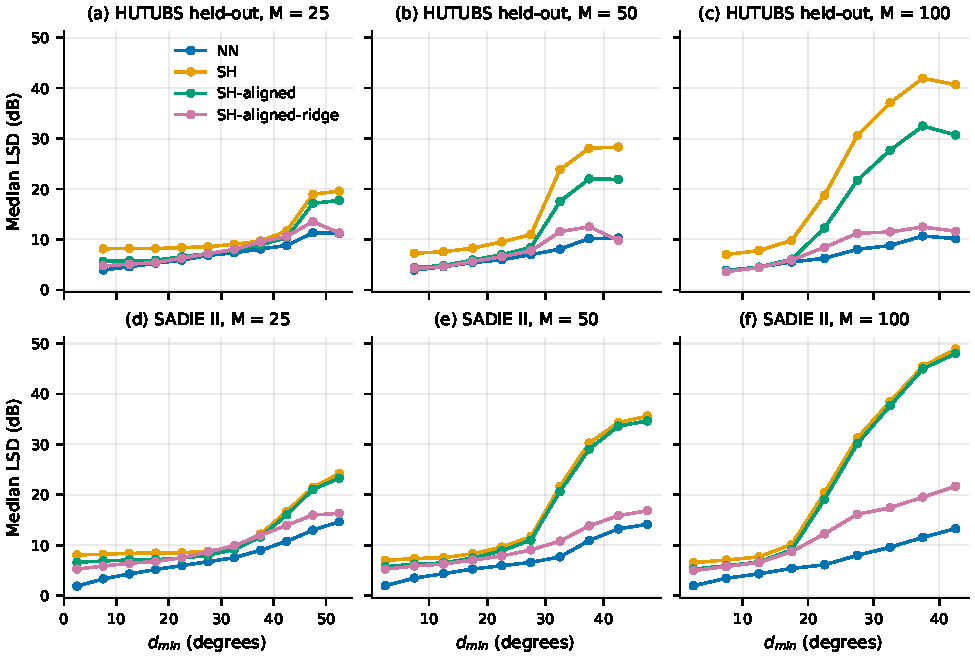
\includegraphics[width=\linewidth]{error_vs_dmin}
\caption{\textbf{Error grows with the distance to the nearest measured direction; for NN and SH the two databases follow the same curve from $5^\circ$ to $30^\circ$.} Median LSD against $\dmin$, pooled over all layouts, budgets and subjects; solid: HUTUBS held-out, dashed: SADIE~II. Bins with fewer than 50 targets are omitted.}
\label{fig:dmin}
\end{figure}

\begin{table}[t]
\centering
\caption{Medians over all layouts, budgets, targets and subjects. SH and SH-aligned use $N_{\mathrm{fit}}$; the ridge methods use the frozen orders. The last two columns are the follow-up with smoothed onsets. Lowest value per row in bold.}
\label{tab:overall}
\footnotesize\setlength{\tabcolsep}{4.2pt}
\begin{tabular}{llcccccc}
\toprule
 & & & & & & \multicolumn{2}{c}{Smoothed onsets (follow-up)} \\
\cmidrule(l){7-8}
Database & Measure & NN & SH & SH-aligned & SH-aligned-ridge & SH-aligned & SH-aligned-ridge \\
\midrule
HUTUBS & LSD 0.2--16~kHz (dB) & \textbf{4.68} & 7.91 & 5.20 & 4.86 & 5.50 & 5.18 \\
 & LSD 8--16~kHz (dB) & \textbf{5.50} & 8.76 & 6.45 & 5.95 & 6.88 & 6.39 \\
 & $|$ITD error$|$ (\textmu s) & 79 & 130 & 14 & 14 & 11 & \textbf{8.5} \\
 & $|$ILD error$|$ (dB) & 2.21 & 4.47 & 1.21 & \textbf{1.09} & 1.35 & 1.21 \\
\midrule
SADIE~II & LSD 0.2--16~kHz (dB) & \textbf{4.41} & 8.01 & 6.89 & 6.57 & 7.03 & 6.68 \\
 & LSD 8--16~kHz (dB) & \textbf{5.16} & 8.75 & 8.12 & 7.65 & 8.49 & 7.96 \\
 & $|$ITD error$|$ (\textmu s) & 68 & 82 & 43 & 43 & \textbf{31} & \textbf{31} \\
 & $|$ILD error$|$ (dB) & \textbf{1.86} & 4.81 & 3.76 & 3.23 & 3.98 & 3.49 \\
\bottomrule
\end{tabular}
\end{table}

NN has the lowest broadband LSD in most conditions (Table~\ref{tab:overall}), because it returns a measured HRTF with all its detail, whereas SH at these orders smooths the detail above $f_A$~\cite{zhang2010,benhur2017}. The advantage is largest on SADIE~II, whose dense grid places 10.3\% of the targets within $5^\circ$ of a context direction (none on HUTUBS). NN pays in its interaural timing: its ITD error on HUTUBS is 5--6 times that of the aligned methods, and its output changes in steps as a source moves (Section~\ref{sec:listening}).

The worst targets follow the covering radius (Figure~\ref{fig:rmax}): across the 12 layouts, its rank correlation with the 95th-percentile LSD is 0.96 (NN) and 0.94 (SH-aligned-ridge) on HUTUBS and 0.95 and 0.78 on SADIE~II, against 0.58--0.63 for the median LSD. Within each budget, $\rmax$ orders the four layouts exactly by their 95th-percentile error on HUTUBS for both methods, and for NN on SADIE~II at $M=25$ and 100, so it flags a poorly covered region even when the median error is low.

\subsection{Conditioning predicts when SH fitting amplifies errors}
\label{sec:kappa}

Across the 72 combinations of layout, budget, grid and order, $N\rmax$ ranks $\log_{10}\kappa$ with $\rho=0.89$, against 0.75 for $N$ alone and 0.05 for $\rmax$ alone. At low orders $\kappa$ is close to 1 and truncation dominates; above $\kappa\approx10$, the median LSD of ordinary SH rises by 5.3~dB per decade on HUTUBS and 6.3~dB on SADIE~II (Figure~\ref{fig:conditioning}a). As \eqref{eq:filter} predicts, the coefficient norm of SH and SH-aligned at $\lambda=0$ grows with $\kappa$ ($\rho=0.78$; median 75 for $\kappa<10$ against 9275 for $\kappa>1000$), and the reconstruction energy relative to the measured HRTFs rises from $-1.6$~dB for $\kappa\le10$ to $+38.3$~dB for $\kappa>1000$ ($\rho=0.91$; Figure~\ref{fig:conditioning}c). The gap layouts reach $\kappa>10^2$ at $N_{\mathrm{fit}}$ for $M=100$ with little change in the median error because their errors stay in the unsampled region (SH: 27.8~dB below $-30^\circ$ against 7.0~dB above).

\begin{figure}[t]
\centering
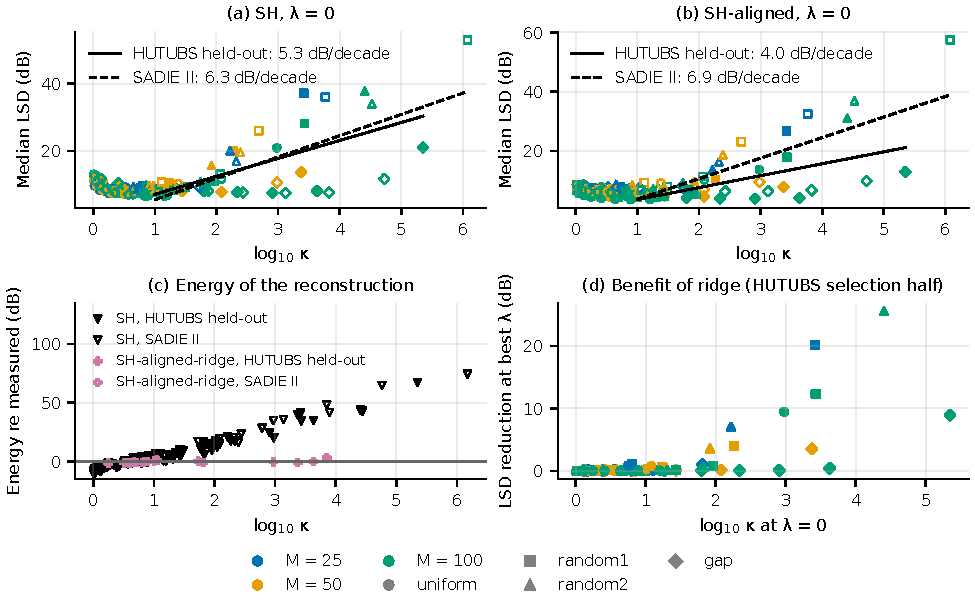
\includegraphics[width=\linewidth]{conditioning}
\caption{\textbf{Above $\kappa\approx10$ the SH fit amplifies errors, and ridge regularisation removes most of the excess.} (a, b) Per-subject median LSD, averaged over subjects, against $\log_{10}\kappa$ at $\lambda=0$, one point per layout, budget and order (filled: HUTUBS held-out; open: SADIE~II); lines are least-squares fits for $\kappa>10$. (c) Reconstruction energy relative to the measured HRTFs. (d) LSD reduction from the best $\lambda$ on the HUTUBS selection half.}
\label{fig:conditioning}
\end{figure}

Ridge regularisation removes most of this rise, and its benefit follows $\kappa$ (Figure~\ref{fig:conditioning}d): on the selection half, the best $\lambda$ lowers the median LSD by 0.15~dB for $10<\kappa\le100$, 2.0~dB for $100<\kappa\le1000$ and 10.6~dB for $\kappa>1000$ (rank correlation 0.84). At $N_{\max}$ the excess error over the best order falls from 8.7 to 0.6~dB, and the reconstruction energy of SH-aligned-ridge stays below $+3.6$~dB. In all 31 cases where ridge lowers the error by more than 0.1~dB, the preferred $\lambda$ is $10^{-2}$ or $10^{-1}$ (Figure~\ref{fig:sv}c). On held-out data at the same order, the frozen $\lambda$ lowers the error by 0.59~dB on HUTUBS and 0.69~dB on SADIE~II; moving from $N_{\mathrm{fit}}$ to the frozen orders costs 0.30 and 0.38~dB at $\lambda=0$, so the net gain over SH-aligned at $N_{\mathrm{fit}}$ is about 0.3~dB in both databases.

\subsection{Transfer from HUTUBS to SADIE~II}
\label{sec:transfer}

All four slopes keep their sign on SADIE~II (Table~\ref{tab:transfer}): three change by 11--19\%, and the $\kappa$ slope of SH-aligned is 72\% steeper (Section~\ref{sec:alignment}). The subject-bootstrap intervals of the two databases do not overlap, so the slopes differ systematically between the databases. The ranking of NN and SH-aligned-ridge agrees in 10 of the 12 conditions: NN has the lower error in all 12 SADIE~II conditions, by 1.7--2.7~dB, and in 10 of 12 on HUTUBS, where four conditions differ by at most 0.05~dB.

\begin{table}[t]
\centering
\caption{Slopes of the error relationships in the two databases. Brackets: 95\% subject-bootstrap intervals.}
\label{tab:transfer}
\footnotesize\setlength{\tabcolsep}{5pt}
\begin{tabular}{llccc}
\toprule
Relationship & Method & HUTUBS held-out & SADIE~II & Change \\
\midrule
LSD vs $\log_{10}\kappa$, $\kappa>10$ (dB/decade) & SH & 5.34 [5.29, 5.38] & 6.34 [6.11, 6.58] & $+19\%$ \\
 & SH-aligned & 4.02 [3.93, 4.12] & 6.93 [6.63, 7.22] & $+72\%$ \\
LSD vs $\dmin$, $\dmin\le35^\circ$ (dB/10$^\circ$) & NN & 1.73 [1.70, 1.77] & 2.03 [1.95, 2.11] & $+17\%$ \\
 & SH-aligned-ridge & 2.17 [2.12, 2.21] & 1.92 [1.83, 2.00] & $-11\%$ \\
\bottomrule
\end{tabular}
\end{table}

The budget alone explains at most 7\% of the per-target variance (Table~\ref{tab:prediction}). Adding $\dmin$ and $\dmin^2$ raises $R^2$ to 0.24--0.47 on HUTUBS, and the HUTUBS models for NN and SH explain 51\% and 32\% of the SADIE~II variance without refitting. $\log_{10}\kappa$ adds four to six points for SH and nothing for SH-aligned-ridge, whose regularisation removes the effect of conditioning. For SH-aligned-ridge the transferred model under-predicts the SADIE~II errors ($R^2=-0.10$), while a refitted model explains 31\%, consistent with the alignment penalty (Section~\ref{sec:alignment}).

\subsection{Time alignment depends on onset quality}
\label{sec:alignment}

On HUTUBS held-out, alignment lowers the median ITD error from 79\us{} (NN) and 130\us{} (SH) to 14\us{}, the 8--16~kHz LSD from 8.8 to 6.5~dB and the error rise from the best order to $N_{\max}$ from 12.5 to 8.5~dB (Table~\ref{tab:overall}, Figure~\ref{fig:alignment}). On SADIE~II the ITD error of SH-aligned is 43\us, the gain above 8~kHz is 0.6~dB and the rise to $N_{\max}$ is unchanged (13.0 against 13.3~dB). An order-3 SH fit to the TOAs of all directions of each subject leaves a per-subject median absolute residual of 7.1\us{} on HUTUBS and 26.5\us{} on SADIE~II on average (Figure~\ref{fig:alignment}b). At 8~kHz, 26\us{} is a fifth of a period, enough to leave the aligned spectra of neighbouring directions partly out of phase, so their interpolation loses high-frequency magnitude. SUpDEq's alignment, which uses a different onset estimator, behaves the same way on SADIE~II (Section~\ref{sec:mca}).

As a follow-up, the context was aligned with the order-3 SH fit of its onsets instead of each direction's own onset, with the same orders and $\lambda$. The ITD error falls from 43 to 31\us{} on SADIE~II and, for SH-aligned-ridge, from 14 to 8.5\us{} on HUTUBS, at a cost of 0.1--0.3~dB in broadband LSD and 0.3--0.4~dB above 8~kHz (Table~\ref{tab:overall}). Removing the measured onsets gives better spectra than removing their smooth trend in both databases, which suggests that the onset variations follow phase variations in the responses; smoothing therefore improves the timing but leaves the spectral gap on SADIE~II in place.

\subsection{Magnitude correction changes the sensitivity to coverage}
\label{sec:mca}

On the SUpDEq subset with identical targets (Table~\ref{tab:mca}), SUpDEq-OBTA and SH-aligned agree within 0.6~dB in broadband and 8--16~kHz LSD, which cross-checks the two implementations; their ITD errors differ on SADIE~II because the onset estimators differ. MCA gives the lowest broadband error on HUTUBS (3.90~dB) and comes within 0.21~dB of NN on SADIE~II, where the other SH methods stay at 6.4--7.3~dB, and it gives the smallest ILD errors (0.74 and 0.90~dB). Its ITD error on SADIE~II stays at 62\us, because magnitude correction does not touch the onsets. SUpDEq reconstructs all targets of one subject and layout in seconds, two to three times longer with magnitude correction, against milliseconds for the Python methods; all are fast enough for offline upsampling.

\begin{figure}[t]
\centering
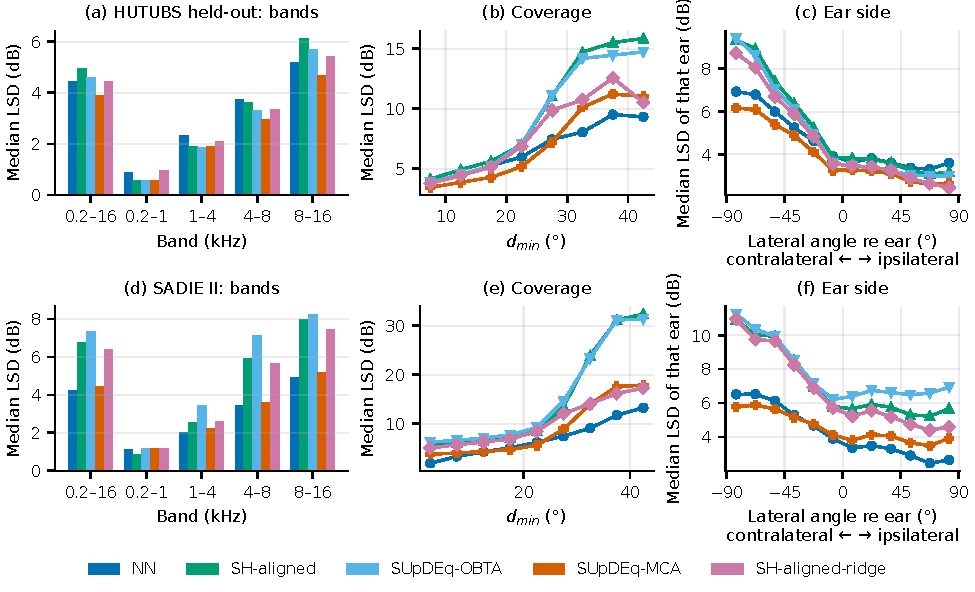
\includegraphics[width=\linewidth]{mca_reference}
\caption{\textbf{Magnitude correction lowers the error most where coverage is poor and on the contralateral side.} SUpDEq subset, identical targets: LSD by band (a, d), LSD against $\dmin$ (b, e) and per-ear LSD against the lateral angle of the source relative to that ear (c, f), for HUTUBS held-out (top) and SADIE~II (bottom).}
\label{fig:mca}
\end{figure}

MCA changes the sensitivity to geometry as well as the average error (Figure~\ref{fig:mca}): at 25--35$^\circ$ from the nearest context direction it gives 8.5~dB against 12.2~dB for OBTA on HUTUBS, and 11.0 against 16.8~dB on SADIE~II. For sources more than $45^\circ$ towards the opposite side of an ear, MCA lowers that ear's LSD from 7.8 to 5.7~dB on HUTUBS and from 10.2 to 5.8~dB on SADIE~II, against reductions of 0.3 and 2.9~dB on the ipsilateral side. In the head shadow the HRTF is weak and detailed, small phase errors between interpolated responses cancel energy, and the correction filter restores it.

\subsection{What the errors look and sound like}
\label{sec:listening}

The horizontal-plane magnitudes (Figure~\ref{fig:plane}) show the same differences: NN holds each measured spectrum over wide azimuth spans, ordinary SH smooths the pinna notches and creates spurious ones, and SH-aligned-ridge and MCA keep the broad pattern, with MCA closest to the measurement on HUTUBS. The listening examples on the project site step pink-noise bursts around the head in 10$^\circ$ steps through the same reconstructions ($M=25$ and 50, one gain per subject): NN changes in steps as the source moves, while the SH-based reconstructions change continuously.

%=====================================================================
\section{Discussion}
\label{sec:discussion}

\subsection{Answer to the research question}

The coverage and conditioning of a sparse layout explain a quarter to a half of the per-target error variance on HUTUBS, and for NN and SH the HUTUBS models also predict the SADIE~II errors without refitting. The distance to the nearest measured direction predicts where the error is large, the covering radius predicts the worst targets, and the condition number predicts when an SH fit amplifies errors and when ridge regularisation is worth using. On SADIE~II these relationships keep their sign and shape; their slopes, and for time-aligned methods the error level, have to be refitted for each measurement chain.

For the secondary question, time alignment makes reconstruction less sensitive to conditioning on HUTUBS (the $\kappa$ slope drops from 5.3 to 4.0~dB per decade) but not on SADIE~II (6.3 against 6.9~dB), while magnitude correction changes the sensitivity to coverage itself, removing 3.7~dB on HUTUBS and 5.8~dB on SADIE~II at 25--35$^\circ$ from the nearest measured direction. The modification, ridge regularisation, controls the amplification where $\kappa$ is large, with a net held-out gain of about 0.3~dB. Spectral accuracy favours NN or MCA, and interaural timing favours aligned SH.

\subsection{Why the descriptors work}

The results show how fast the error grows with distance from the data, give the same curve in two measurement chains and explain several times more variance than the number of directions, the quantity usually reported. The distance $\dmin$ measures how well a target is covered, which matters most at high frequencies, where the HRTF changes quickly with direction~\cite{zhang2010}, and $\rmax$ describes the single largest gap and therefore the tail of the error distribution. SH adds truncation, which smooths detail above $f_A$, and extrapolation, which turns the SH curves upwards beyond about $35^\circ$ (Figure~\ref{fig:dmin}). When the largest gap is too wide for the order, \eqref{eq:filter} divides by small singular values and the reconstruction gains energy the HRTF does not have; ridge regularisation removes this amplification but cannot supply missing data, so the unsampled region of the gap layout stays poorly reconstructed (Figure~\ref{fig:maps}).

\subsection{Comparison with published results}

Bau et al.\ found that the optimal SH order on sparse irregular grids depends mainly on the grid and the regularisation~\cite{bau2022}; the transfer of the $\kappa$ and $\dmin$ relationships to a second measurement chain is consistent with that finding and extends it from the choice of order to the error at each direction. They also found every fit stable for $\kappa<10$, the boundary found here, and judged $\kappa$ unsuitable for choosing the order; here $\kappa$ instead flags amplification and the need for regularisation. Zotkin et al.\ applied regularised SH fitting to incomplete grids~\cite{zotkin2009}; the present results show when it pays off ($\kappa>100$) and that one range, $\lambda=0.01$--$0.1$, serves all tested layouts once the basis is orthonormal and the weights are normalised. The HUTUBS results match the lower required order after alignment reported by Arend et al.~\cite{arend2021}, and the weaker benefit on SADIE~II matches the sensitivity of estimated delays noted by Ben-Hur et al.~\cite{benhur2019}. Arend et al.\ found that MCA improves high frequencies by up to 1.5~dB over all directions and 4~dB contralaterally on simulated HRTFs~\cite{arend2023}; on the measured HRTFs here it improved the 8--16~kHz LSD by 1.0~dB (HUTUBS) and 3.1~dB (SADIE~II) over OBTA and the contralateral LSD by 2.1 and 4.4~dB. Absolute values differ because~\cite{arend2023} used dense simulated HUTUBS data on controlled grids, but the pattern is the same.

The known differences between databases~\cite{andreopoulou2015,wen2023} enter here through the onsets and the error levels, while the geometric relationships keep their form. The descriptors also complement learned interpolation: $\dmin$ and $\rmax$ give a cheap, subject-independent counterpart, available before the first measurement, to the calibrated uncertainty of Thuillier et al.~\cite{thuillier2024}.

\subsection{Sources of error and limitations}

The evaluation is objective: a sagittal-plane localisation model such as that of Baumgartner et al.~\cite{baumgartner2014}, available in the Auditory Modeling Toolbox~\cite{majdak2022amt}, would show how the spectral differences affect localisation, and a short listening test how the LSD and ITD differences are perceived. The two databases also differ in distance (1.47 and 1.2~m) and equalisation; a third database such as SONICOM~\cite{engel2023} and the frequency-response normalisation of~\cite{wen2023} would separate these factors from sampling. A common uniform target set would remove the advantage NN gains on SADIE~II, whose denser grid places more targets close to the context. Running MCA on all 63 test subjects instead of ten would confirm the ear-side gain. The Python methods use one onset estimator, while ITD estimators are known to disagree~\cite{katz2014}; the parametric ear alignment of~\cite{benhur2019} would remove the dependence on onset estimates. The linear models leave 50--75\% of the per-target variance unexplained; a per-subject term, the target elevation or frequency-dependent descriptors could capture part of it.

\subsection{Lessons learned}

If the project were started again, the onset and coordinate checks, which decided the onset rule and the elevation limit, would come before any layout is designed. The most useful tool learned was the singular-value decomposition of the SH matrix, which shows before any measurement which spatial patterns a set of measurement positions can resolve.

%=====================================================================
\section{Conclusion}

The sampling geometry of a sparse HRTF measurement predicts where and when reconstruction becomes unreliable, and the form of this prediction carries over from HUTUBS to SADIE~II, while its slopes, and for time-aligned methods its level, have to be refitted. Because the descriptors are known before any measurement, a planned layout can be screened in milliseconds: map the directions onto the measurement grid, compute $\dmin$, $\rmax$ and $\kappa$, prefer the layout with the smaller $\rmax$, keep $N\rmax$ small and use $\lambda=0.01$--$0.1$ whenever $\kappa$ exceeds about 100. After measuring, check the smoothness of the onsets before relying on time alignment; where the residual is large, MCA keeps its benefit, most on the contralateral side, and smoothed onsets improve the ITD at a small spectral cost. The next steps are to optimise layouts directly against $\rmax$ and $\kappa$, to compare the descriptors with the uncertainty of learned interpolators and to confirm the differences perceptually.

%=====================================================================

\begingroup
\small
\setlength{\itemsep}{0.5pt}
\begin{thebibliography}{99}
\bibitem{li2020} S.~Li and J.~Peissig, ``Measurement of head-related transfer functions: A review,'' \emph{Appl. Sci.}, vol.~10, no.~14, art.~5014, 2020, doi:10.3390/app10145014.
\bibitem{evans1998} M.~J. Evans, J.~A.~S. Angus, and A.~I. Tew, ``Analyzing head-related transfer function measurements using surface spherical harmonics,'' \emph{J. Acoust. Soc. Am.}, vol.~104, no.~4, pp.~2400--2411, 1998, doi:10.1121/1.423749.
\bibitem{duraiswami2004} R.~Duraiswami, D.~N. Zotkin, and N.~A. Gumerov, ``Interpolation and range extrapolation of HRTFs,'' in \emph{Proc. IEEE Int. Conf. Acoust., Speech, Signal Process. (ICASSP)}, vol.~4, 2004, doi:10.1109/ICASSP.2004.1326759.
\bibitem{romigh2015} G.~D. Romigh, D.~S. Brungart, R.~M. Stern, and B.~D. Simpson, ``Efficient real spherical harmonic representation of head-related transfer functions,'' \emph{IEEE J. Sel. Topics Signal Process.}, vol.~9, no.~5, pp.~921--930, 2015, doi:10.1109/JSTSP.2015.2421876.
\bibitem{benhur2019} Z.~Ben-Hur, D.~L. Alon, R.~Mehra, and B.~Rafaely, ``Efficient representation and sparse sampling of head-related transfer functions using phase-correction based on ear alignment,'' \emph{IEEE/ACM Trans. Audio, Speech, Lang. Process.}, vol.~27, no.~12, pp.~2249--2262, 2019, doi:10.1109/TASLP.2019.2945479.
\bibitem{arend2021} J.~M. Arend, F.~Brinkmann, and C.~P\"orschmann, ``Assessing spherical harmonics interpolation of time-aligned head-related transfer functions,'' \emph{J. Audio Eng. Soc.}, vol.~69, no.~1/2, pp.~104--117, 2021, doi:10.17743/jaes.2020.0070.
\bibitem{arend2023} J.~M. Arend, C.~P\"orschmann, S.~Weinzierl, and F.~Brinkmann, ``Magnitude-corrected and time-aligned interpolation of head-related transfer functions,'' \emph{IEEE/ACM Trans. Audio, Speech, Lang. Process.}, vol.~31, pp.~3783--3799, 2023, doi:10.1109/TASLP.2023.3313908.
\bibitem{thuillier2024} E.~Thuillier, C.~T. Jin, and V.~V\"alim\"aki, ``HRTF interpolation using a spherical neural process meta-learner,'' \emph{IEEE/ACM Trans. Audio, Speech, Lang. Process.}, vol.~32, pp.~1790--1802, 2024, doi:10.1109/TASLP.2024.3361377.
\bibitem{bau2022} D.~Bau, J.~M. Arend, and C.~P\"orschmann, ``Estimation of the optimal spherical harmonics order for the interpolation of head-related transfer functions sampled on sparse irregular grids,'' \emph{Front. Signal Process.}, vol.~2, art.~884541, 2022, doi:10.3389/frsip.2022.884541.
\bibitem{andreopoulou2015} A.~Andreopoulou, D.~R. Begault, and B.~F.~G. Katz, ``Inter-laboratory round robin HRTF measurement comparison,'' \emph{IEEE J. Sel. Topics Signal Process.}, vol.~9, no.~5, pp.~895--906, 2015, doi:10.1109/JSTSP.2015.2400417.
\bibitem{wen2023} Y.~Wen, Y.~Zhang, and Z.~Duan, ``Mitigating cross-database differences for learning unified HRTF representation,'' in \emph{Proc. IEEE Workshop Appl. Signal Process. Audio Acoust. (WASPAA)}, 2023, pp.~1--5, doi:10.1109/WASPAA58266.2023.10248178.
\bibitem{brinkmann2019} F.~Brinkmann, M.~Dinakaran, R.~Pelzer, P.~Grosche, D.~Voss, and S.~Weinzierl, ``A cross-evaluated database of measured and simulated HRTFs including 3D head meshes, anthropometric features, and headphone impulse responses,'' \emph{J. Audio Eng. Soc.}, vol.~67, no.~9, pp.~705--718, 2019, doi:10.17743/jaes.2019.0024.
\bibitem{armstrong2018} C.~Armstrong, L.~Thresh, D.~Murphy, and G.~Kearney, ``A perceptual evaluation of individual and non-individual HRTFs: A case study of the SADIE II database,'' \emph{Appl. Sci.}, vol.~8, no.~11, art.~2029, 2018, doi:10.3390/app8112029.
\bibitem{supdeq} AudioGroupCologne, ``SUpDEq: Spatial Upsampling by Directional Equalization,'' MATLAB toolbox, commit 877401f, May 2025. [Online]. Available: \url{https://github.com/AudioGroupCologne/SUpDEq}
\bibitem{wightman1992} F.~L. Wightman and D.~J. Kistler, ``The dominant role of low-frequency interaural time differences in sound localization,'' \emph{J. Acoust. Soc. Am.}, vol.~91, no.~3, pp.~1648--1661, 1992, doi:10.1121/1.402445.
\bibitem{jin2004} C.~Jin, A.~Corderoy, S.~Carlile, and A.~van Schaik, ``Contrasting monaural and interaural spectral cues for human sound localization,'' \emph{J. Acoust. Soc. Am.}, vol.~115, no.~6, pp.~3124--3141, 2004, doi:10.1121/1.1736649.
\bibitem{algazi2001} V.~R. Algazi, R.~O. Duda, D.~M. Thompson, and C.~Avendano, ``The CIPIC HRTF database,'' in \emph{Proc. IEEE Workshop Appl. Signal Process. Audio Acoust. (WASPAA)}, 2001, pp.~99--102, doi:10.1109/ASPAA.2001.969552.
\bibitem{jin2014} C.~T. Jin, P.~Guillon, N.~Epain, R.~Zolfaghari, A.~van Schaik, A.~I. Tew, C.~Hetherington, and J.~Thorpe, ``Creating the Sydney York morphological and acoustic recordings of ears database,'' \emph{IEEE Trans. Multimedia}, vol.~16, no.~1, pp.~37--46, 2014, doi:10.1109/TMM.2013.2282134.
\bibitem{engel2023} I.~Engel, R.~Daugintis, T.~Vicente, A.~O.~T. Hogg, J.~Pauwels, A.~J. Tournier, and L.~Picinali, ``The SONICOM HRTF dataset,'' \emph{J. Audio Eng. Soc.}, vol.~71, no.~5, pp.~241--253, 2023, doi:10.17743/jaes.2022.0066.
\bibitem{majdak2022} P.~Majdak, F.~Zotter, F.~Brinkmann, J.~De~Muynke, M.~Mihocic, and M.~Noisternig, ``Spatially Oriented Format for Acoustics 2.1: Introduction and recent advances,'' \emph{J. Audio Eng. Soc.}, vol.~70, no.~7/8, pp.~565--584, 2022, doi:10.17743/jaes.2022.0026.
\bibitem{zhang2010} W.~Zhang, T.~D. Abhayapala, R.~A. Kennedy, and R.~Duraiswami, ``Insights into head-related transfer function: Spatial dimensionality and continuous representation,'' \emph{J. Acoust. Soc. Am.}, vol.~127, no.~4, pp.~2347--2357, 2010, doi:10.1121/1.3336399.
\bibitem{rafaely2019} B.~Rafaely, \emph{Fundamentals of Spherical Array Processing}, 2nd~ed. Cham, Switzerland: Springer, 2019, doi:10.1007/978-3-319-99561-8.
\bibitem{benhur2017} Z.~Ben-Hur, F.~Brinkmann, J.~Sheaffer, S.~Weinzierl, and B.~Rafaely, ``Spectral equalization in binaural signals represented by order-truncated spherical harmonics,'' \emph{J. Acoust. Soc. Am.}, vol.~141, no.~6, pp.~4087--4096, 2017, doi:10.1121/1.4983652.
\bibitem{mhaskar2001} H.~N. Mhaskar, F.~J. Narcowich, and J.~D. Ward, ``Spherical Marcinkiewicz--Zygmund inequalities and positive quadrature,'' \emph{Math. Comput.}, vol.~70, no.~235, pp.~1113--1130, 2001, doi:10.1090/S0025-5718-00-01240-0.
\bibitem{zotkin2009} D.~N. Zotkin, R.~Duraiswami, and N.~A. Gumerov, ``Regularized HRTF fitting using spherical harmonics,'' in \emph{Proc. IEEE Workshop Appl. Signal Process. Audio Acoust. (WASPAA)}, 2009, pp.~257--260, doi:10.1109/ASPAA.2009.5346521.
\bibitem{porschmann2019} C.~P\"orschmann, J.~M. Arend, and F.~Brinkmann, ``Directional equalization of sparse head-related transfer function sets for spatial upsampling,'' \emph{IEEE/ACM Trans. Audio, Speech, Lang. Process.}, vol.~27, no.~6, pp.~1060--1071, 2019, doi:10.1109/TASLP.2019.2908057.
\bibitem{katz2014} B.~F.~G. Katz and M.~Noisternig, ``A comparative study of interaural time delay estimation methods,'' \emph{J. Acoust. Soc. Am.}, vol.~135, no.~6, pp.~3530--3540, 2014, doi:10.1121/1.4875714.
\bibitem{zhang2023} Y.~Zhang, Y.~Wang, and Z.~Duan, ``HRTF field: Unifying measured HRTF magnitude representation with neural fields,'' in \emph{Proc. IEEE Int. Conf. Acoust., Speech, Signal Process. (ICASSP)}, 2023, pp.~1--5, doi:10.1109/ICASSP49357.2023.10095801.
\bibitem{spharpy} pyfar project, ``spharpy,'' Python package, version 1.0.1, 2026. [Online]. Available: \url{https://github.com/pyfar/spharpy}
\bibitem{hansen1998} P.~C. Hansen, \emph{Rank-Deficient and Discrete Ill-Posed Problems: Numerical Aspects of Linear Inversion}. Philadelphia, PA, USA: SIAM, 1998, doi:10.1137/1.9780898719697.
\bibitem{kuhn1955} H.~W. Kuhn, ``The Hungarian method for the assignment problem,'' \emph{Naval Res. Logist. Q.}, vol.~2, no.~1--2, pp.~83--97, 1955, doi:10.1002/nav.3800020109.
\bibitem{hutubs} F.~Brinkmann, M.~Dinakaran, R.~Pelzer, J.~J. Wohlgemuth, F.~Seipel, D.~Voss, P.~Grosche, and S.~Weinzierl, ``The HUTUBS head-related transfer function (HRTF) database,'' Technische Universit\"at Berlin, 2019, dataset, doi:10.14279/depositonce-8487.
\bibitem{sadie} AudioLab and G.~C. Kearney, ``SADIE II Database,'' version 2-2, AudioLab, University of York, 2024, dataset, doi:10.5281/zenodo.12092466.
\bibitem{gonzalez2010} \'A.~Gonz\'alez, ``Measurement of areas on a sphere using Fibonacci and latitude--longitude lattices,'' \emph{Math. Geosci.}, vol.~42, no.~1, pp.~49--64, 2010, doi:10.1007/s11004-009-9257-x.
\bibitem{slaney1998} M.~Slaney, ``Auditory Toolbox, Version 2,'' Interval Research Corporation, Tech. Rep. 1998-010, 1998.
\bibitem{baumgartner2014} R.~Baumgartner, P.~Majdak, and B.~Laback, ``Modeling sound-source localization in sagittal planes for human listeners,'' \emph{J. Acoust. Soc. Am.}, vol.~136, no.~2, pp.~791--802, 2014, doi:10.1121/1.4887447.
\bibitem{majdak2022amt} P.~Majdak, C.~Hollomey, and R.~Baumgartner, ``AMT 1.x: A toolbox for reproducible research in auditory modeling,'' \emph{Acta Acust.}, vol.~6, art.~19, 2022, doi:10.1051/aacus/2022011.
\end{thebibliography}
\endgroup

%=====================================================================
\appendix
\section{Additional Figures and Tables}
\setcounter{figure}{0}\setcounter{table}{0}
\renewcommand{\thefigure}{A\arabic{figure}}\renewcommand{\thetable}{A\arabic{table}}

\begin{figure}[H]
\centering
\begin{tikzpicture}[
  font=\scriptsize, >={Stealth[length=1.8mm]},
  box/.style={draw, rounded corners=2pt, align=center, inner sep=2.5pt, line width=0.5pt},
  geo/.style={box, fill=blue!6, draw=blue!55!black},
  sig/.style={box, fill=orange!9, draw=orange!70!black},
  pro/.style={box, fill=black!5, draw=black!55, minimum height=10mm},
  fol/.style={box, dashed, fill=white, draw=black!55, minimum height=10mm},
  title/.style={font=\footnotesize\bfseries},
  lab/.style={font=\scriptsize\bfseries, text=black!65, anchor=south west, inner sep=0pt}]
  % row 1: signal path, repeated for every subject, layout and budget
  \node[sig, text width=29mm, minimum height=25mm] (data) at (15mm,0) {{\footnotesize\bfseries Measured HRIRs}\\[2pt]HUTUBS: 94 sets\\SADIE~II: 18 subjects\\[2pt]onset rule\\elevation $\ge-65^\circ$};
  \node[geo, text width=37mm, minimum height=25mm] (layout) at (53mm,0) {{\footnotesize\bfseries Sparse layout}\\[2pt]
    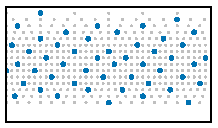
\includegraphics[width=16mm]{inset_uniform}\hspace{1.5mm}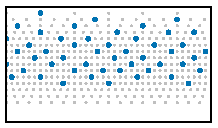
\includegraphics[width=16mm]{inset_gap}\\[1pt]
    uniform, random1, random2, gap\\$M = 25, 50, 100$ directions};
  \node[sig, text width=33mm, minimum height=25mm] (rec) at (95.5mm,0) {{\footnotesize\bfseries Reconstruction}\\[2pt]NN, SH, SH-aligned,\\SH-aligned-ridge\\[2pt]SUpDEq OBTA and MCA\\(ten-subject subset)};
  \node[sig, text width=29mm, minimum height=25mm] (err) at (135mm,0) {{\footnotesize\bfseries Errors per target}\\[2pt]LSD in five bands\\and per ear\\[2pt]$|\Delta\mathrm{ITD}|$, $|\Delta\mathrm{ILD}|$};
  % row 2: geometry path
  \node[geo, text width=37mm, minimum height=11mm] (desc) at (53mm,-21mm) {{\footnotesize\bfseries Layout descriptors}\\[1pt]$d_{\min}$ per target; $r_{\max}$; $\kappa(N)$};
  \node[geo, text width=29mm, minimum height=11mm] (ana) at (135mm,-21mm) {{\footnotesize\bfseries Analysis}\\[1pt]error against descriptors};
  \draw[->] (data) -- (layout);
  \draw[->] (layout) -- (rec);
  \draw[->] (rec) -- (err);
  \draw[->] (layout) -- (desc);
  \draw[->] (err) -- (ana);
  \draw[->] (desc) -- node[above]{same analysis in both databases} (ana);
  \node[lab] at ([yshift=1.3mm]data.north west) {Repeated for every subject, layout and budget};
  % row 3: protocol
  \node[pro, text width=34mm] (sel) at (17mm,-38mm) {Select $N$ and $\lambda$ on the\\HUTUBS selection half (49)};
  \node[pro, text width=19mm] (frz) at (51.5mm,-38mm) {Freeze the\\configuration};
  \node[pro, text width=40mm] (test) at (92mm,-38mm) {Apply unchanged to HUTUBS\\held-out (45) and SADIE~II (18)};
  \node[fol, text width=29mm] (fol) at (135mm,-38mm) {Follow-up: smoothed onsets,\\ear side, run time, demo};
  \draw[->] (sel) -- (frz);
  \draw[->] (frz) -- (test);
  \draw[->, dashed] (test) -- (fol);
  \node[lab] at ([yshift=1.3mm]sel.north west) {Protocol};
\end{tikzpicture}

\caption{\textbf{Study design.} Top: the path repeated for every subject, layout and budget; insets show the uniform and gap layouts with $M=50$ (blue) on the HUTUBS grid (grey). Bottom: the protocol; the follow-up experiments ran after the frozen test.}
\label{fig:overview}
\end{figure}

\begin{table}[H]
\centering
\caption{Data and protocol. Directions are those with elevation $\ge-65^\circ$.}
\label{tab:data}
\footnotesize
\setlength{\tabcolsep}{5pt}
\begin{tabularx}{\linewidth}{@{}lXX@{}}
\toprule
 & HUTUBS (measured) & SADIE~II (v2-2) \\
\midrule
Subjects; directions & 94 sets (pp2--pp95); 418 & 18 humans (H3--H20); 2561 (H3--H9) or 1921 (H10--H20) \\
Distance; format & 1.47~m; 44.1~kHz, 256 taps & 1.2~m; 44.1~kHz, 256 taps \\
Role & 49 sets select $N$ and $\lambda$ (pp2--pp6 and even IDs); 45 held out (odd IDs from pp7) & External test with the frozen configuration \\
SUpDEq subset & pp7, pp9, pp11, pp13, pp15 & H3, H7, H11, H15, H19 \\
\bottomrule
\end{tabularx}
\end{table}

\begin{figure}[H]
\centering
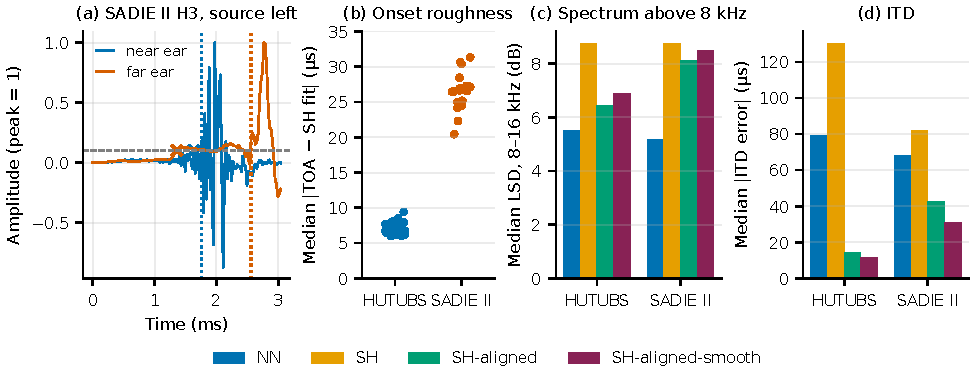
\includegraphics[width=\linewidth]{alignment}
\caption{\textbf{Alignment helps where the onsets are smooth.} (a) SADIE~II H3, source at azimuth $90^\circ$, each ear normalised to its peak: the far ear's slow rise crosses the 10\% threshold (dashed) first (crosses), while the high-pass rule (dotted) finds the correct order. (b) Per-subject median residual of an order-3 SH fit to the onset times. (c, d) Median 8--16~kHz LSD and ITD error over all layouts and budgets; SH-aligned-smooth is the follow-up with smoothed onsets.}
\label{fig:alignment}
\end{figure}

\begin{figure}[H]
\centering
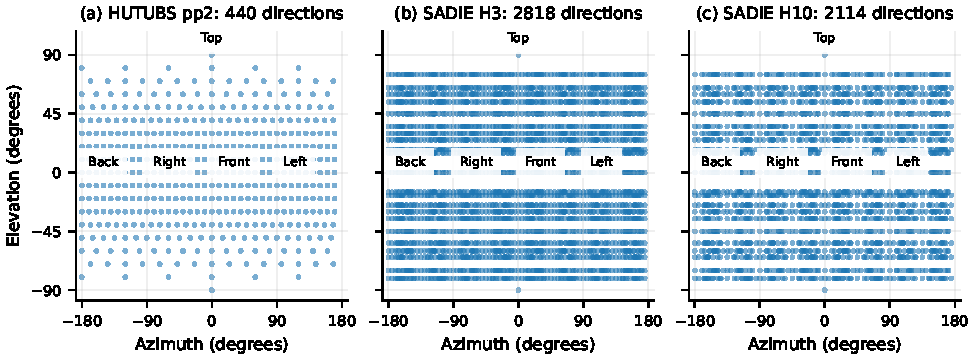
\includegraphics[width=\linewidth]{measured_directions}\\[2pt]
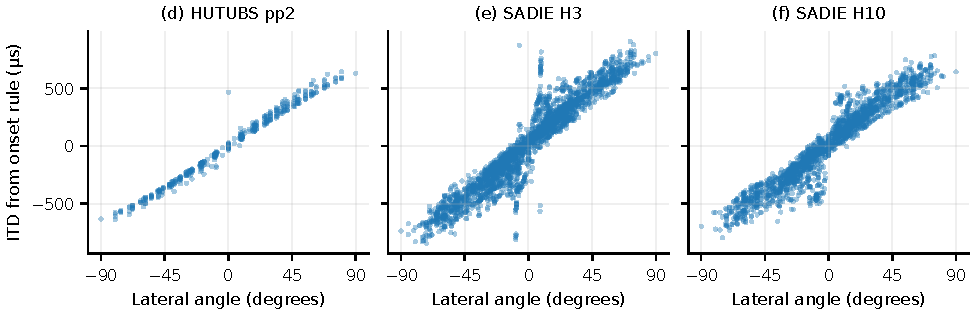
\includegraphics[width=\linewidth]{itd_vs_lateral}
\caption{\textbf{Grids and onset check.} Measured directions of the three grid types before the elevation limit, with front, left, back, right and top marked (a--c), and the ITD from the high-pass onset rule against lateral angle over all directions (d--f).}
\label{fig:appendix}
\end{figure}

\begin{table}[H]
\centering
\caption{Realisation of the $M=100$ layouts on the three grid types. Mapping error: angle between each nominal direction and its measured direction; NN spacing: angle from each context direction to its nearest other context direction. Angles in degrees.}
\label{tab:geometry}
\footnotesize\setlength{\tabcolsep}{4pt}
\begin{tabular}{llccccc}
\toprule
 & & Mapping error & NN spacing & & \multicolumn{2}{c}{$\kappa$} \\
\cmidrule(lr){3-3}\cmidrule(lr){4-4}\cmidrule(l){6-7}
Layout & Grid & mean / median / max & median / max & $\rmax$ & $N_{\mathrm{fit}}=6$ & $N_{\max}=9$ \\
\midrule
uniform & HUTUBS & 3.8 / 3.9 / 6.4 & 14.5 / 21.4 & 15.1 & 4.4 & $9.6{\times}10^{2}$ \\
 & SADIE~II H3 & 2.7 / 2.3 / 7.4 & 17.4 / 20.4 & 16.5 & 3.7 & $1.4{\times}10^{2}$ \\
 & SADIE~II H10 & 3.0 / 2.8 / 7.4 & 17.3 / 19.9 & 15.5 & 3.7 & $1.1{\times}10^{2}$ \\
\midrule
random1 & HUTUBS & 3.6 / 3.7 / 8.3 & 10.0 / 22.0 & 30.7 & 10.1 & $2.7{\times}10^{3}$ \\
 & SADIE~II H3 & 2.8 / 2.6 / 8.1 & 10.1 / 24.9 & 35.2 & 11.4 & $7.1{\times}10^{5}$ \\
 & SADIE~II H10 & 3.0 / 2.9 / 8.1 & 10.3 / 24.9 & 34.7 & 11.4 & $1.5{\times}10^{6}$ \\
\midrule
random2 & HUTUBS & 3.8 / 4.0 / 7.9 & 10.0 / 20.7 & 22.4 & 7.9 & $2.6{\times}10^{4}$ \\
 & SADIE~II H3 & 2.7 / 2.3 / 7.8 & 9.8 / 22.3 & 23.4 & 6.5 & $4.3{\times}10^{4}$ \\
 & SADIE~II H10 & 2.9 / 2.6 / 8.0 & 10.0 / 22.3 & 23.4 & 7.8 & $2.8{\times}10^{4}$ \\
\midrule
gap & HUTUBS & 3.8 / 3.9 / 6.7 & 13.9 / 20.7 & 40.1 & 218 & $2.2{\times}10^{5}$ \\
 & SADIE~II H3 & 2.8 / 2.4 / 7.4 & 15.0 / 19.4 & 42.9 & 253 & $4.4{\times}10^{4}$ \\
 & SADIE~II H10 & 3.0 / 2.6 / 7.4 & 15.1 / 19.6 & 43.3 & 276 & $5.8{\times}10^{4}$ \\
\bottomrule
\end{tabular}
\end{table}

\begin{figure}[H]
\centering
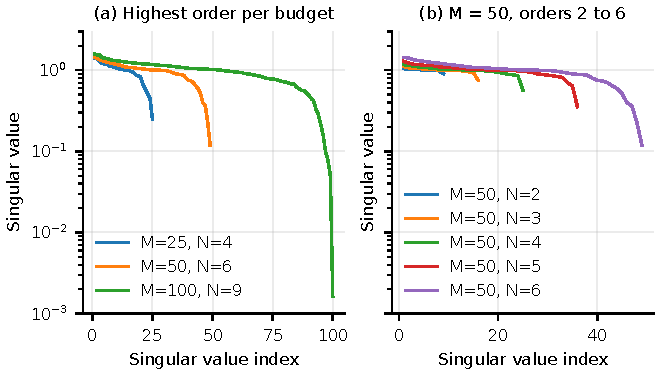
\includegraphics[width=0.64\linewidth]{singular_values}\hfill
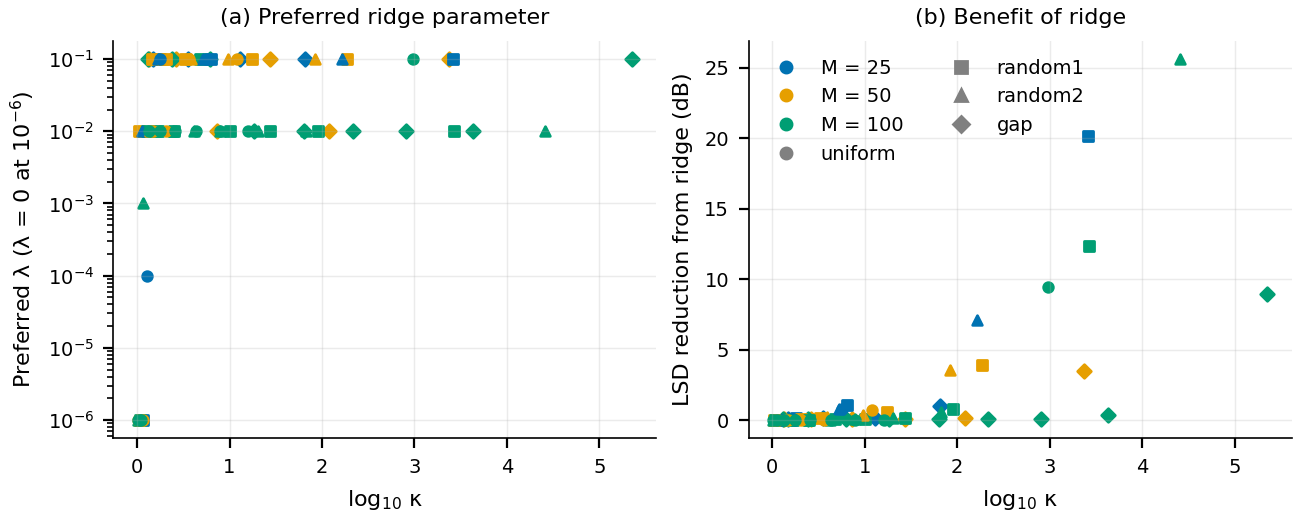
\includegraphics[width=0.34\linewidth]{lambda_vs_kappa}
\caption{\textbf{Singular values and the preferred ridge parameter.} (a, b) Singular values of $\mathbf W^{1/2}\mathbf Y$ for the uniform HUTUBS layouts at their highest order and for $M=50$ at orders 2 to 6: the last singular values collapse only at the highest order. (c) Preferred ridge parameter on the HUTUBS selection half, one point per layout, budget and order; colours and markers as in Figure~\ref{fig:conditioning}.}
\label{fig:sv}
\end{figure}

\begin{figure}[H]
\centering
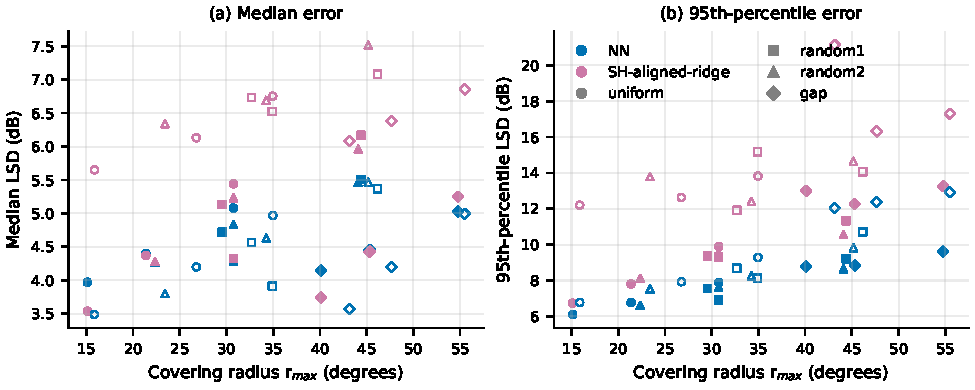
\includegraphics[width=\linewidth]{error_vs_rmax}
\caption{\textbf{The covering radius ranks the 95th-percentile error better than the median error.} Median (a) and 95th-percentile (b) LSD against $\rmax$, one point per layout and budget; per-subject values averaged over subjects. Filled: HUTUBS held-out; open: SADIE~II.}
\label{fig:rmax}
\end{figure}

\begin{table}[H]
\centering
\caption{Variance of per-target LSD explained by linear models fitted on HUTUBS held-out ($R^2$). Transferred: HUTUBS coefficients applied to SADIE~II, an out-of-sample prediction on the same nominal layouts; HUTUBS and refitted values are in-sample. $M$: budget indicators. SH at $N_{\mathrm{fit}}$.}
\label{tab:prediction}
\footnotesize\setlength{\tabcolsep}{5pt}
\begin{tabular}{llccc}
\toprule
Method & Predictors & HUTUBS & SADIE~II, transferred & SADIE~II, refitted \\
\midrule
NN & $M$ & 0.06 & 0.05 & 0.06 \\
 & $M$, $\dmin$, $\dmin^2$ & 0.47 & 0.51 & 0.54 \\
\midrule
SH & $M$ & 0.00 & $-0.01$ & 0.00 \\
 & $M$, $\dmin$, $\dmin^2$ & 0.24 & 0.32 & 0.39 \\
 & $M$, $\dmin$, $\dmin^2$, $\log_{10}\kappa$ & 0.30 & 0.36 & 0.43 \\
\midrule
SH-aligned-ridge & $M$ & 0.07 & $-0.32$ & 0.01 \\
 & $M$, $\dmin$, $\dmin^2$ & 0.34 & $-0.10$ & 0.31 \\
\bottomrule
\end{tabular}
\end{table}

\begin{table}[H]
\centering
\caption{SUpDEq subset (5 + 5 subjects, uniform and gap layouts, $M=25/50/100$), medians over identical targets. Contra./ipsi.: per-ear LSD for sources more than $45^\circ$ towards the opposite or the same side of that ear. Run time: median wall-clock time to reconstruct all targets of one subject and layout on an Apple M2 (Python: median of five runs; SUpDEq in MATLAB: after one untimed warm-up call). Lowest value per row in bold.}
\label{tab:mca}
\footnotesize\setlength{\tabcolsep}{4.2pt}
\begin{tabular}{llccccc}
\toprule
Database & Measure & NN & SH-aligned & SUpDEq-OBTA & SUpDEq-MCA & SH-aligned-ridge \\
\midrule
HUTUBS & LSD 0.2--16~kHz (dB) & 4.46 & 4.94 & 4.60 & \textbf{3.90} & 4.45 \\
 & LSD 8--16~kHz (dB) & 5.20 & 6.12 & 5.71 & \textbf{4.67} & 5.42 \\
 & LSD contra./ipsi. (dB) & 6.39/3.37 & 8.19/3.22 & 7.80/3.02 & \textbf{5.74}/\textbf{2.70} & 7.42/2.76 \\
 & LSD at $\dmin=25$--$35^\circ$ (dB) & \textbf{7.73} & 12.86 & 12.20 & 8.53 & 10.39 \\
 & $|$ITD error$|$ (\textmu s) & 79 & \textbf{11} & \textbf{11} & 14 & \textbf{11} \\
 & $|$ILD error$|$ (dB) & 2.12 & 1.22 & 0.98 & \textbf{0.74} & 0.92 \\
\midrule
SADIE~II & LSD 0.2--16~kHz (dB) & \textbf{4.22} & 6.74 & 7.31 & 4.43 & 6.37 \\
 & LSD 8--16~kHz (dB) & \textbf{4.92} & 7.99 & 8.24 & 5.18 & 7.47 \\
 & LSD contra./ipsi. (dB) & 6.30/\textbf{2.74} & 10.00/5.29 & 10.15/6.54 & \textbf{5.75}/3.60 & 9.74/4.62 \\
 & LSD at $\dmin=25$--$35^\circ$ (dB) & \textbf{8.10} & 16.15 & 16.81 & 11.03 & 12.80 \\
 & $|$ITD error$|$ (\textmu s) & 65 & \textbf{37} & 60 & 62 & \textbf{37} \\
 & $|$ILD error$|$ (dB) & 1.78 & 3.73 & 4.47 & \textbf{0.90} & 3.14 \\
\midrule
Run time & HUTUBS (368 targets) & 0.7~ms & 22~ms & 0.52~s & 1.49~s & 27~ms \\
 & SADIE~II (1896 targets) & 4.2~ms & 58~ms & 2.41~s & 5.48~s & 69~ms \\
\bottomrule
\end{tabular}
\end{table}

\begin{figure}[H]
\centering
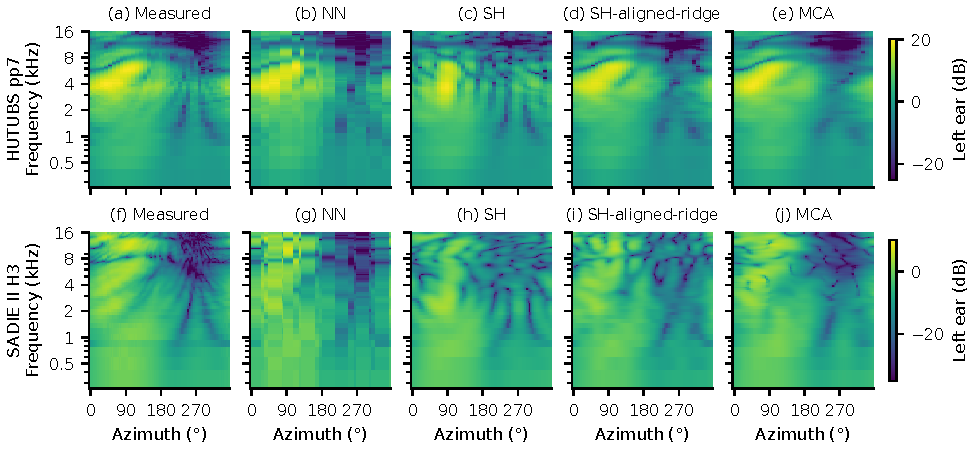
\includegraphics[width=\linewidth]{hrtf_horizontal_plane}
\caption{\textbf{Left-ear magnitude on the horizontal plane.} Measured and reconstructed from the uniform layout with $M=50$, for HUTUBS pp7 (a--e) and SADIE~II H3 (f--j); azimuth runs counter-clockwise from the front ($90^\circ$ = left). The listening examples use the same reconstructions.}
\label{fig:plane}
\end{figure}

\FloatBarrier
\section*{AI Use Acknowledgement}
AI was involved in preparing this report, mainly for language polishing, code generation and implementation, and the integration of ideas.

\end{document}
